\documentclass{article}
\usepackage{graphicx}
\usepackage{tikz}
\usepackage{amsmath}
\title{Sample Project}
\author{Phi}
\date{\today}

\begin{document}
\maketitle

\section{Introduction}
Hello from the sample project. Euler's identity: $e^{i\pi} + 1 = 0$.

\begin{center}

\includegraphics[width=0.2\linewidth]{favicon.png}
\end{center}

\section{Fibonacci Sequence}
The Fibonacci sequence is defined by the recurrence relation $F_n = F_{n-1} + F_{n-2}$, typically starting with $F_0 = 0$ and $F_1 = 1$. The sequence begins: 0, 1, 1, 2, 3, 5, 8, 13, 21, \dots

\section{Navier--Stokes Equations}
The incompressible Navier--Stokes equations describe the motion of fluid substances:
\begin{align}
\frac{\partial \mathbf{u}}{\partial t} + (\mathbf{u} \cdot \nabla) \mathbf{u} &= -\frac{1}{\rho} \nabla p + \nu \nabla^2 \mathbf{u} + \mathbf{f}, \\
\nabla \cdot \mathbf{u} &= 0,
\end{align}
where $\mathbf{u}$ is the velocity field, $p$ is the pressure, $\rho$ is the density, $\nu$ is the kinematic viscosity, and $\mathbf{f}$ represents external forces. The first equation expresses conservation of momentum, and the second enforces incompressibility.

\subsection{chapter 1}
tadaeaze

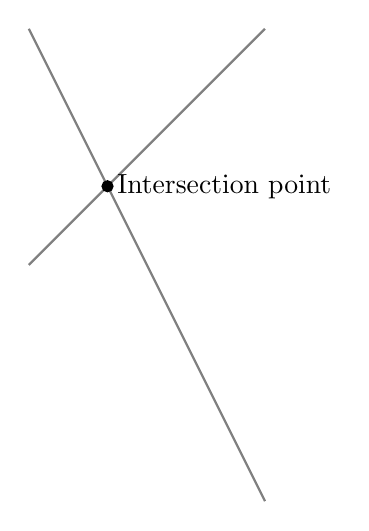
\begin{tikzpicture}
\draw[gray, thick] (-1,2) -- (2,-4);
\draw[gray, thick] (-1,-1) -- (2,2);
\filldraw[black] (0,0) circle (2pt) node[anchor=west]{Intersection point};
\end{tikzpicture}
\end{document}


\end{document}
